\documentclass[
oneside,
12pt, % The default document font size, options: 10pt, 11pt, 12pt
%oneside, % Two side (alternating margins) for binding by default, uncomment to switch to one side
english, % ngerman for German
doublespacing, % Single line spacing, alternatives: onehalfspacing or doublespacing
%draft, % Uncomment to enable draft mode (no pictures, no links, overfull hboxes indicated)
%nolistspacing, % If the document is onehalfspacing or doublespacing, uncomment this to set spacing in lists to single
%liststotoc, % Uncomment to add the list of figures/tables/etc to the table of contents
%toctotoc, % Uncomment to add the main table of contents to the table of contents
%parskip, % Uncomment to add space between paragraphs
%nohyperref, % Uncomment to not load the hyperref package
headsepline, % Uncomment to get a line under the header
chapterinoneline, % Uncomment to place the chapter title next to the number on one line
%consistentlayout, % Uncomment to change the layout of the declaration, abstract and acknowledgements pages to match the default layout
]{MastersDoctoralThesis} % The class file specifying the document structure

\usepackage[utf8]{inputenc} % Required for inputting international characters
\usepackage[T1]{fontenc} % Output font encoding for international characters

% \usepackage{mathpazo} % Use the Palatino font by default
\usepackage{times}
%\usepackage[backend=bibtex,style=authoryear,natbib=true]{biblatex}
% Use the bibtex backend with the authoryear citation style (which resembles APA)
%\addbibresource{amycao.bib} % The filename of the bibliography

\usepackage{apacite}
\usepackage{natbib}
\usepackage[autostyle=true]{csquotes} % Required to generate language-dependent quotes in the bibliography

\usepackage{graphicx}
\usepackage{hyperref}

\usepackage[colorinlistoftodos]{todonotes}
%\usepackage{ulem}
\usepackage[normalem]{ulem}
\usepackage{textcomp}
\usepackage{subcaption}
\usepackage{booktabs}
\usepackage{multirow}
\usepackage{amsmath}
\usepackage{url}
\usepackage{changepage}
\usepackage[toc,page]{appendix}
\usepackage[export]{adjustbox}
\usepackage{nopageno}

\newcommand{\specialcell}[2][c]{%
  \begin{tabular}[#1]{@{}c@{}}#2\end{tabular}}
\newcommand{\ra}[1]{\renewcommand{\arraystretch}{#1}}

%function strikeout

\linespread{1.2}
%----------------------------------------------------------------------------------------
%	MARGIN SETTINGS
%----------------------------------------------------------------------------------------

\geometry{
	paper=a4paper, % Change to letterpaper for US letter
	inner=5cm, % Inner margin
	outer=2cm, % Outer margin
	bindingoffset=.5cm, % Binding offset
	top=2.5cm, % Top margin
	bottom=2.5cm, % Bottom margin
	%showframe, % Uncomment to show how the type block is set on the page
}
\setcounter{tocdepth}{4}
\setcounter{secnumdepth}{3}
%----------------------------------------------------------------------------------------
%	THESIS INFORMATION
%----------------------------------------------------------------------------------------
% \submitdate{April, 2018}
% \commencementyear{2018}

\begin{document}

\frontmatter % Use roman page numbering style (i, ii, iii, iv...) for the pre-content pages

\pagestyle{plain} % Default to the plain heading style until the thesis style is called for the body content

%----------------------------------------------------------------------------------------
%	TITLE PAGE
%----------------------------------------------------------------------------------------
\begin{titlepage}
\newgeometry{bottom=3cm}
        \thispagestyle{empty}
   \begin{adjustwidth}{-3cm}{-3cm}



\begin{center}

\vspace*{.06\textheight}

\HRule \\[0.3cm] % Horizontal line
{\huge \bfseries
Wie Mutterschaft beeinflusst die Fähigkeit \\der Inhibitionskontrolle \\
\vspace{0.2cm}
\Large Eine empirische Studie über
        eine erweiterte Stroop Aufgabe \par}\vspace{0.3cm} % Thesis title
%{\Large \bfseries ----Eine empirische Studie über eine erweiterte Stroop Aufgabe\par}\vspace{0.4cm}
\HRule \\[3cm] % Horizontal line

\textsc{\Large Bachelor Arbeit}\\[0.3cm] % Thesis type
        {\large in der Fachrichtung Psychologie}\\
[0.3cm]
{\large der \Large Universität des Saarlandes}\\
[1.5cm]
{\normalsize vorgelegt von}\\
[0.2cm]
{\Large Yuexin Cao}\\
[1.5cm]
Betreuer: Prof. Sommer and Dr. Recio\\
[0.5cm]
Erstgutachter:\\ Prof. Mecklinger\\
[0.5cm]
Zweitprüfer:\\ Prof. Wentura\\


\vfill
%\vspace{\fill}
{\large \scshape Saarbrücken 2018}
%{\large \today}\\[4cm] % Date
\end{center}
\end{adjustwidth}
\end{titlepage}

\let\cleardoublepage\clearpage

%\begin{acknowledgements}
%\end{acknowledgements}


% \tableofcontents % Prints the main table of contents

% \listoffigures % Prints the list of figures

% \listoftables % Prints the list of tables


\mainmatter % Begin numeric (1,2,3...) page numbering

\pagestyle{thesis} % Return the page headers back to the "thesis" style

% Include the chapters of the thesis as separate files from the Chapters folder
% Uncomment the lines as you write the chapters

\addchap{Abstract}

The concept ``social character'', first defined by Erich Fromm, describes the common emotional attitudes and psychological reactions to people in a social class or in a society~\citep{fromm1941escape}. 

inspired by the concept, David Riesman wrote the book ``The Lonely Crowd'', who is a sociologist and a social critic as well, and has a
major influence on American cultural life. In this book, three social characters based on the American society are identified, where individuals are classified as the members of different characters. Namely, the tradition-directed members obey the rules; the inner-directed members are akin to follow the inner gyroscope; and the other-directed members tend to go after the peers and mass media~\citep{riesman2001lonely}. 

Among this three categories, the other-directed members, who are particularly influenced externally rather than internally, are often criticized for their conformity~\citep{mcclay1998lonely}. In this article, I argue that some of such criticisms are not objective enough and tend to interpret the conformity pessimistically. To bridge the gap, the concept of the conformity is first introduced and then analyzed in the context of each three social character. Besides, some positive aspects of the other-direct character are highlighted as well as their costs. Thereafter, the solution for the conformity, a fourth social character of the changing society, namely, the autonomous, is introduced, where the difficulty and feasibility to achieve the autonomy in the other-directed world are further discussed. 




\chapter{Introduction}\label{chp.introduction}

As a theoretical sociologist, Erich Fromm first defined the concept ``social character'' by integrating Marx's theory concerning how the mode of production determines ideology with Freud's concept of character. Instead of the common emotional attitudes and psychological reactions to people of an individual, ``social character'' is defined as ones in a social class or society~\citep{fromm1941escape}. 

Influenced by Erich Fromm personally and intellectually, David Riesman considered the concept ``social character'' in the context of the American society and identified three types of social characters in his book ``The Lonely Crowd'', first published in 1950 as a sociological analysis of American life. Surprisingly, it soon became a bestseller and is considered by many to be the most influential book of the twentieth century, resulting in the concerns of people all over the world, especially of Americans, about the changing of the social character.

The three types of the social characters based on the American society are the tradition-directed, the inner-directed and the other-directed type. Additionally, the transitions between them are also introduced in this book~\citep{riesman2001lonely}. The society with high birth rate and high death rate was dominated by the tradition-directed type, whose members tend to stick to the rules. As the death rate declines, the social character shifted from the inner-directed type to the other-directed one, whose members akin to behave according to their own inner gyroscope implanted by elders. As the birth rate began to follow the death rate downward, the social character shifted from the inner-directed type in 19th-century to the other-directed type in the mid-20th-century, whose members become very sensitive to the preferences and expectations of others.

The intention of ``The Lonely Crowd'' was primarily to analyze the American life rather than to point with anxiety to its deficiencies, however, as the sociologist Dennis H. Wrong observed, ``it was widely read as deploring the rise of the psychological disposition called `other-direction' at the expense of `inner-direction'. '' The conformity of the other-directed people, who have little autonomous and seem to follow the trend all the time, is often criticized by the readers. 

%As the source of ``evil'', the culture are severe criticized as well, especially the informative and interactive social media, inducing the public to become more other-directed and to go conformity, while misleading and disorienting them at the same time.

However, the conformity is actually necessary for the changing society, ensuring the normal functioning of it. Each of the three types of social characters has the conformity trend, differing in to whom and how, which is not unique in the other-directed type. Moreover, the other-directed member seems to be more autonomous than the other-directed person, but is no less a conformist to others, since they are akin to listen to the old generations.

As economists often say, everything has a price. The cost of the transition from an inner-directed type to an other-directed type is not so bad as many thought. The positive aspects of the other-direct character, namely, openness and flexibility should not be overlooked, although it may lead to the anxiety about what to do and whom to trust.

In terms of the concerns about the conformity, the solution for the conformity, a fourth social character of the changing society, namely, the autonomous is introduced, whose members are capable of conforming to the behavioral norms of their society but are free to choose whether to conform or not. However, there are many challenges to become an autonomous person, for example, the anxiety when we face the uncertainty, and the impact of the mass media, making the conformity much easier and reasonable. To achieve autonomy in an other-directed world, one should have confidence in himself as well as the self-awareness, while think critically to the large amounts of information.
 
The chapters are sketched as follows. The work begins with the background in Chapter~\ref{chp.background} including the introduction of the main author, David Riesman, and his work ``The Lonely Crowd'' in Section~\ref{chp.background.david} as well as the definitions of three types of the social characters in Section~\ref{chp.background.characters}. In Chapter~\ref{chp.Criticism}, the statements about the other-directed type in the book are listed in~\ref{chp.Criticism.Book}, while in the Section~\ref{chp.Criticism.Readers}, some well-known critics about the conformity of other-directed people from readers are introduced. In Chapter~\ref{chp.reinterpretation}, the conformities of each three characters are introduced in Section~\ref{chp.reinterpretation} at the very beginning, indicating that the conformity does not exist only in the other-directed type. Thereafter, the advantages and the costs of being a other-directed type are introduced respectively in Section~\ref{chp.reinterpretation.advantage} and~\ref{chp.reinterpretation.cost}. In Chapter~\ref{chp.solution}, a solution in terms of the conformity of the other-directed type is introduced, namely, autonomous. In Chapter~\ref{chp.discussion}, the work is summarized and the autonomous is discussed in the context of the modern society.


\chapter{Background}\label{chp.background}
In this Chapter, the book which this work based on, ``The Lonely Crowd'' and its author David Riesman are introduced in the Section~\ref{chp.background.david}. As the main part of the book, the definition and characteristics of the concept ``social character'' are first introduced, based on the works from Erich Fromm. Afterwards, three social characters, identified by David Riesman are introduced in Section~\ref{chp.background.characters}. 

\section{David Riesman and His Work}\label{chp.background.david}

David Riesman was a sociologist, educator, and best-selling commentator on American society. Born to a wealthy German Jewish family in 1909, he graduated from Harvard College with a degree in biochemistry in 1931, then earned his law degree from Harvard Law School. Afterwards, he taught at the University of Buffalo Law School and at the University of Chicago. In the late 1940s, he took a leave from Chicago to focus on a project at Yale, which sponsored the work that led to ``The Lonely Crowd''. In 1958, he left Chicago for a
position as University Professor at Harvard, where he
remained for the rest of his teaching career and passed by in 2002.

As the most famous work of David Riesman, the book ``The Lonely Crowd'', first published in 1950 as a sociological analysis of American life, became a surprising bestseller and is considered to be the most influential book of the twentieth century~\citep{riesman1979making}. According to~\citeauthor{horowitz2010david}, It is also the nation’s most influential and widely read mid-century work of social and cultural criticism and catapulted its author to the cover of Time magazine in 1954, making David Riesman the first social scientist so honored~\citep{horowitz2010david}. As historian
Rupert Wilkinson suggests, ```The Lonely Crowd' heralded later findings to a degree that is seldom appreciated. Narcissism
and `diffuse anxiety'; the shifting of authority from `dos and don'ts' to manipulation and enticement; the flooding of attitudes by media messages; the channeling of achievement drives into competition for the approval of others; and the splintering of society into myriad interest groups--all these tendencies of modern American life that so worried commentators in the 1970s and 80s were spotted by Riesman et al.''~\citep{wilkinson1988pursuit}. In the book, following topics are mainly introduced and discussed.
\begin{itemize}
\item[1] Three social characters and their different characteristics.%which will be shortly introduced in Section~\ref{chp.background.characters}.  
\item[2] The way different social characters prevail in the work, in leisure, in politics and in education. %In this work, the influence of the other-directed type is introduced in Section~\ref{chp.Criticism.Book}.  
\item[3] The transition of the social characters, namely, a gradual replacement by a social character of a completely different kind.% which is introduced in ~\ref{chp.background.characters} and~\ref{chp.Criticism.Comparison}.
\item[4] Why and how this replacement took place and how it affects some major areas of life.
\end{itemize}
 
\section{Social characters and Transitions}\label{chp.background.characters}  

\textbf{Erich Fromm.}
The social character is the central basic concept of the analytic social psychology of Erich Fromm, who was a German psychoanalyst, sociologist and former member of the Institute for
Social Research in Frankfurt. The concept integrates Marx's theory concerning how the mode of production determines ideology with Freud's concept of character~\citep{fromm1941escape}.

While individual character describes the richness of the character structure of an individual, the social character describes the common of the emotional attitudes and psychological reactions to people in a social class or society. In particular, the concept describes the formation of the shared character structure of the people of a society or a social class according to their way of life, the socially typical expectations and functional requirements regarding socially adaptive behavior. The social character is necessary to be acquired and obeyed by the members of a society, enabling their members to do what they need to do in order to prosper and enabling a society to function adequately~\citep{fromm1941escape, fromm1994escape}.

Although everyone develops character traits and character orientations that distinguish them from people who live in other cultures, people in every culture with the same mode of production share basic elements of the social character~\citep{fromm1970social}, making it possible to generate the social character in one culture to other cultures. For example, three social characters based on the American society in the book ``The Lonely Crowd'' are not limited in the United States but also have a certain reference value to other cultures, which could explain, in some degree, why the book became the best-seller all over the world.

\textbf{David Riesman.}~As a patient of the therapist Erich Fromm in the early 1940s, David Riesman was influenced intellectually and personally, due to an unconventional psychoanalysis, which resembles a teacher/student rather than a psychoanalyst/patient relationship, resulting in his interest in sociology and further extension of the concept ``social character'' in his work ``the Lonely Crowd''. In the book, three types of social characters: the tradition-directed, the inner-directed, and the other-directed type are identified and analyzed as well as the transitions between them.

\begin{figure}{t!}
  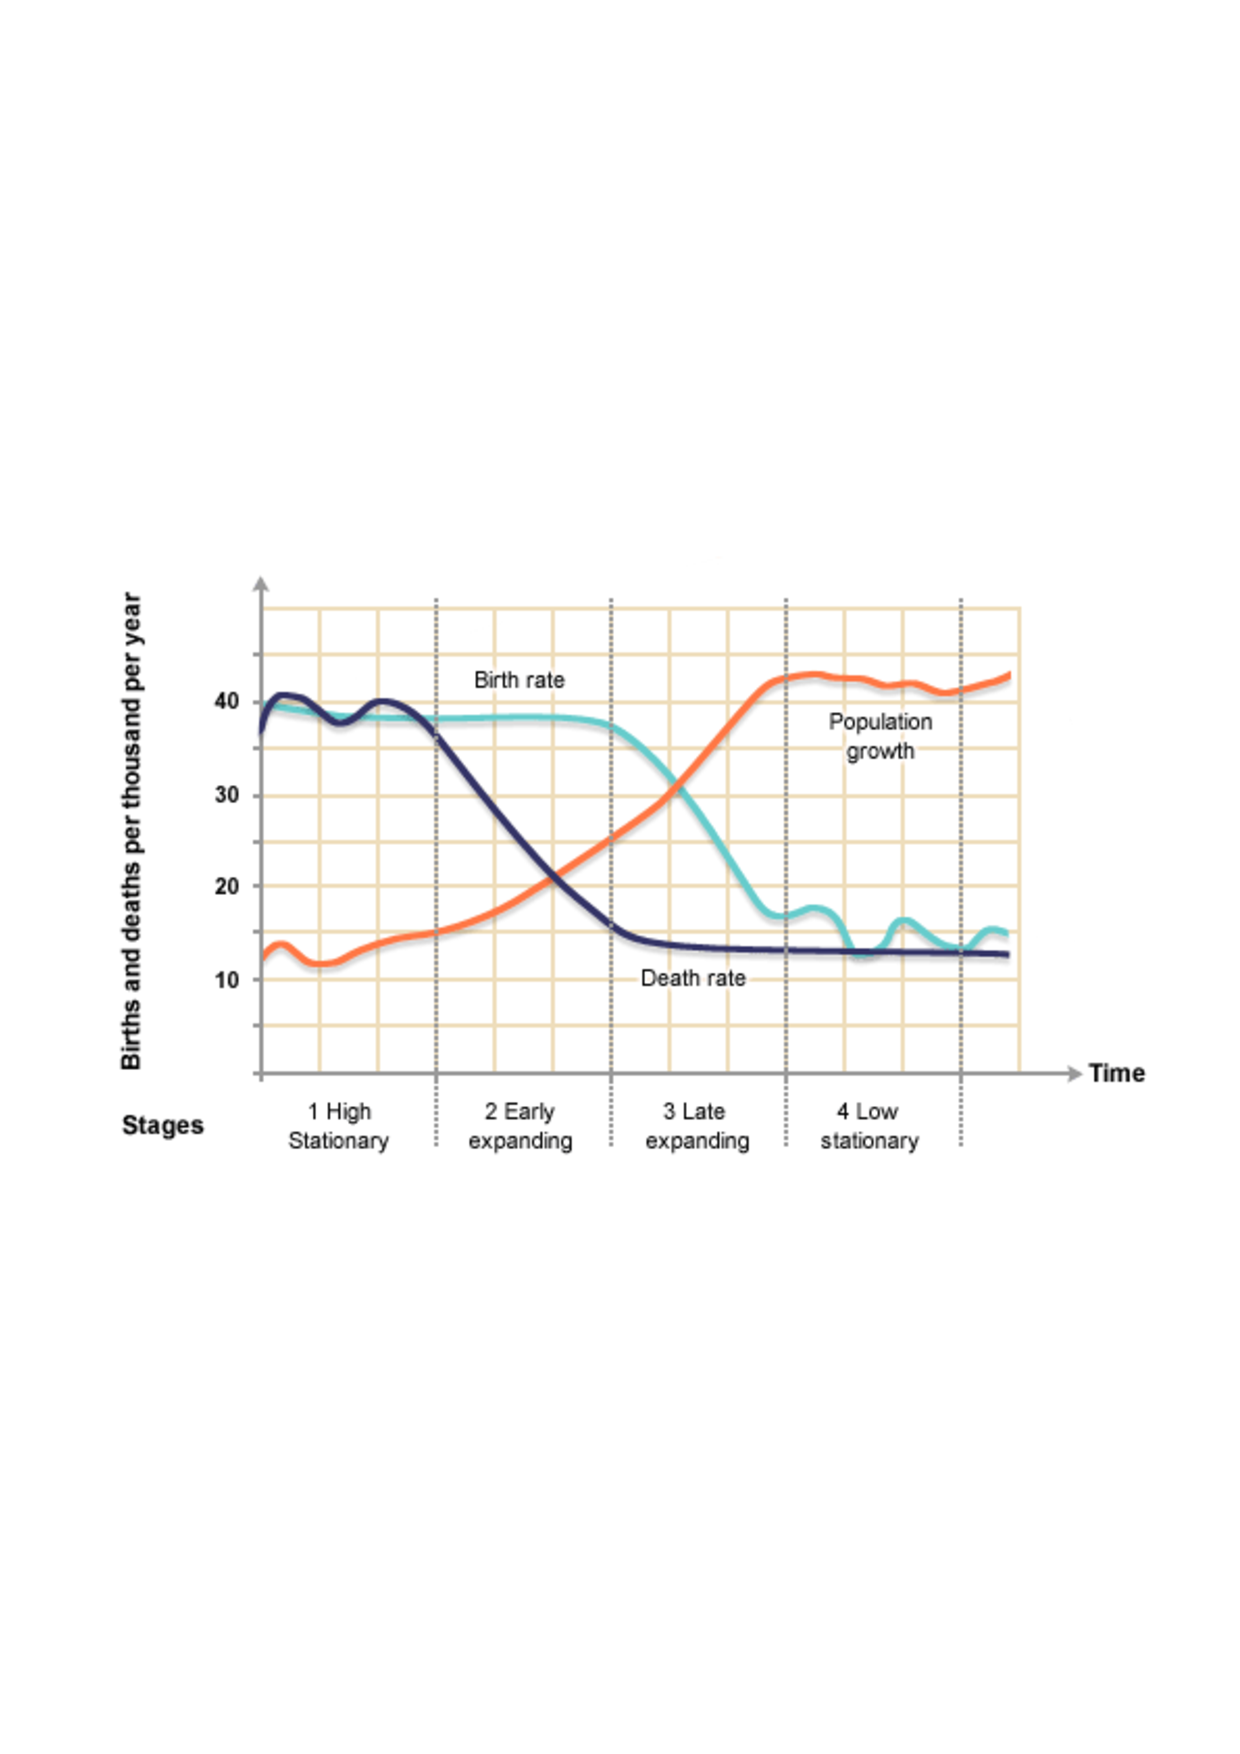
\includegraphics[width=\linewidth]{population_changes.pdf}
  \caption{The changes in the birth and death rates as well as the population growth during the transitions}
  \label{background.fig.population}
\end{figure}


\textbf{The tradition-directed type} dominates in the primitive societies, where both birth rate and death rate were high (refers to the first stage in Figure~\ref{background.fig.population}). Its members are with a low level of individualism and strong ties to primary groups, obeying rules established a long time in the past. This kind of social character has, according to Riesman, disappeared in the modern American
society, except in pockets of black, French Canadian, Southern, rural and immigrant cultures. 

Due to the drop of death rate in industrial economies (refers to the second stage in Figure~\ref{background.fig.population}), as well as industrialization, urbanization and modern technology, there was an intensive expansion of goods and people. As a result, many novel situations were presented, where a strict code could not encompass in advance like in the tradition-directed society and the control of the primary group in a tradition directed society was loosened. Therefore,~\textbf{the inner-directed type} became dominant, offering a wide choice but stable at the same time, whose members discovered the potential within themselves to live and act not according to the established norms but based on what they discovered using their own inner gyroscope that were essentially ``implanted'' by elders. Compared to the other-directed type, the inner-directed type of social character is focused on producing than consuming, whose members conform their outward behaviors, like dressing, to match societal norms, while the opinions of others have little sway on their inner lives, for example, the goal of pursuing money and rights. In other words, They would rather be esteemed than be loved.

In the mid twenties century, as the birth rate begins to follow the death rate downward (refers to the third and fourth stage in Figure~\ref{background.fig.population}), societies move toward the epoch of incipient decline of population and of service, trade and communications-driven economy. Fewer and fewer people work, hours are short, people may have material abundance and leisure besides, who are mixed more widely and thereafter becoming more sensitive to each other, since material environment is no longer a problem. Therefore, the social character was shifting from a 19th-century inner-directed type to a mid-20th-century~\textbf{other-directed type}, dominated by a concern for ``niceness'' instead of achievement, leisure instead of competition and ``consumerism'' instead of production. However, due to the lack of the cultural expectations for how to live, the other-directed people look to their peers and the media for guidance, making them very sensitive to the preferences and expectations of others using a ``radar''. Compared to inner-directed people, they would rather be loved than esteemed. In particular, modern parents and teachers are anxiety ridden as their authority over children and students has been undermined by the media, youth culture and a rapid social change that creates a situation where the ``other-directed child is often more knowing than his parents''. 


			

			
		



\chapter{Criticisms on Other-directed and its Conformity}\label{chp.Criticism}

The transition from the inner-directed type of society to the other-directed type with a ``stronger'' conformity has led to the discussions and concerns of many American readers. In this chapter, the descriptions of the conformity in the other-directed people in the book are introduced in Section~\ref{chp.Criticism.Book}, resulting in the interpretation and criticisms over the other-directed type of society, which are introduced in Section~\ref{chp.Criticism.Readers}.

\section{Conformity of Other-directed In the Book}\label{chp.Criticism.Book}

Conformity is the extent to which an individual complies with group norms or expectations. Erich Fromm defined the ``automation conformity'' as a mechanism of a human being in his work ``The Fear of Freedom'', which could be seen as an extreme case of the conformity. Having the automation conformity, an individual ceases to be himself and adopts entirely the kind of personality offered to him by cultural patterns, becoming exactly as all others are and as they expect him to be. This mechanism can be compared with the protective coloring some animals assume, looking so similar to their surroundings, being hardly distinguishable. As a result, the discrepancy between ``I'' and the world, with the conscious fear of aloneness and powerlessness disappears, namely, the person who gives up his individual self and becomes an automaton, identical with millions of other automatons around him, does not need to feel alone and anxious any more. But the price he pays, however, is high, namely, the loss of his self~\citep{fromm1941fear}.

Recall the descriptions in the book ``The Lonely Crowd'', other-directed people are easily influenced by the peer groups and mass media~\ref{chp.background.characters}, which induce them to conform due to the peer pressure, whose influence is not only external, such as dress, act but also internal, such as thoughts and emotions. Similarly to the description of the automation conformity~\citep{fromm1941fear}, the conformity of the other-directed people also leads to following the trend, namely, wearing a uniform, belonging and thinking uniform thoughts. Because they are afraid of being different, standing out or taking a stand on important issues. Thereafter the group of contemporaries, comrades and colleagues play a very important role in their life. Different from the disappear of the aloneness and powerlessness after the conformity, indicated by Erich Fromm~\citep{fromm1941fear}, David Riesman suggested that having lost touch with themselves, other-directed souls were actually alone in the midst of other people, therefore, as donated from the name of the book, feel lonely. Moreover, society dominated by the other-directed people also faces profound deficiencies in leadership, individual self-knowledge, and human potential. 

\section{Interpretation and Criticisms by Readers}\label{chp.Criticism.Readers}
Along with Erich Fromm’s ``Escape from Freedom''~\citep{fromm1941escape}, William H. Whyte Jr.’s ``The Organization Man''~\citep{whyte2002organization} and Vance Packard’s ``The Status Seekers''~\citep{packard1959status}, most of the reading public and many critics saw ``The Lonely Crowd'' more narrowly, who links the autonomy and inner-direction closely, as ``a great secular jeremiad against other-direction''~\citep{mcclay1998lonely} and as part of the social pessimism which is fashionable in this period, arguing that the society is heading in the wrong direction~\citep{steenvoorden2016societal}. 

Due to the fast development of the social networks, such as Facebook and Twitter, more and more people worry about how mass media threatens individualism by promoting conformity. For example, children no longer care much about the authority of adults but are rather hyperalert to the peer groups and gripped by mass media, which is sometimes incorrect and misleading. ``Father might know best, but if he did, it was increasingly because a television program said so.'' At the meantime, the adults read the commends of an affair on the newspaper or in the Internet, then chatted with their colleagues without thinking on their own. 





\chapter{Reinterpretation Outer-directed Character}\label{chp.reinterpretation}
As the criticisms and interpretations from the readers introduced in Chapter~\ref{chp.Criticism} are incomplete and relative pessimistic, in this chapter, the conformity of each three types of the social characters as well as the criticisms over the inner-directed type are introduced in the Section~\ref{chp.reinterpretation.conformity}. The descriptions of the other-directed type is then interpreted from a more objective and complete perspective, including the advantages in Section~\ref{chp.reinterpretation.advantage} and costs in Section~\ref{chp.reinterpretation.cost}.

\section{Conformity of Three Characters}\label{chp.reinterpretation.conformity}

In terms of conformity, the other-directed type of social character should not be specifically criticized, referring to the reasons stated in the following. 

% However, the conformity in the other-directed people, who use the peers and mass media to assess and understand how to act, to dress, and to behave, caused the most anxiety and was heatedly discussed.

First of all, such conformity tendency could be found in all three types of social character, which differs in to whom and how. Moreover, conformity is necessary and essential in forming the social character and in ensuring the normal functioning of the changing society. What David Riesman actually suggested was that, society could be thought in terms of a series of ``ideal types'' along a spectrum of increasingly loose authority and with different kinds of conformity, whereas, not conforming may lead to a a specific emotion corresponded to each social character.

\noindent - \textbf{Tradition-directed}\\
On one end of the spectrum is the ``tradition-directed'' community, where its members all understand that what they should to do is what they are supposed to do. Authority is unequivocal and there is neither the room nor the desire for autonomous action. Accordingly, tradition-directed people conform with the rules and regulations. The primary disciplining emotion under tradition direction is shame, the threat of ostracism and exile that enforces the traditional action.\\

\noindent - \textbf{Inner-directed}\\ 
In the middle of the spectrum, as one moves toward a freer distribution of the authority, is ``inner-direction''. The inner-directed person is concerned not with ``what one does'' but with ``what people tell me to do''. Put differently, he looks to his own internalizations of past authorities to get a sense for how to conduct his affairs, seeking after tangible goals, such as cars, house, wealth, which were the symbols of success, told by the gyroscopes planted by his parents. When not conforming, he experiences guilt instead of shame, and the fear that his behavior won’t be commensurate with the imago within.\\

\noindent - \textbf{Other-directed}\\
On the other end of the spectrum is the ``other-directed'' community, also known as the contemporary society, where the inculcated authority of the vertical (one’s lineage) gives way to the muddled authority of the horizontal (one’s peers), namely, its members look right and left instead of up and down. Compared to the inner-directed people, the other-directed one seek experiences over stuff, which could be seen as a better aim. However, their drive towards these experiences does not come from their own, but from watching other people. Therefore, the other-directed people do not just conform to others as far as external behavior, but also seek to match the quality of other people’s inner experience, looking to others for ``what experiences to seek and in how to interpret them''. In short, other-directed people conform with the thoughts (internal) and behaviors (external) from the mass media and peers. When not conforming, they experience a ``contagious, highly diffuse'' anxiety instead of guilty, and the possibility that they might be doing the wrong thing all the time, due to the fact that the authority itself is diffuse and ambiguous. 

That is to say, David Riesman drew no moral from the transition from a community of primarily inner-directed people to a community of the other-directed ones. Instead, he saw that each ideal type had different advantages and faced different problems. Moreover, when comparing the inner-directed member and other-directed one, whose characters are introduced in the~\ref{chp.background.characters}, the former does not consult some deep and subjective internal voices, instead, it consults the internalized voices of a mostly dead lineage, while the latter heeds the external voices of her living contemporaries. As is indicated by Riesman, ``the gyroscopic mechanism allows the inner-directed person to appear far more independent than he really is: he is no less a conformist to others than the other-directed person, but the voices to which he listens are more distant, of an older generation, their cues internalized in his childhood''. The inner-directed person is, simply, ``somewhat less concerned than the other-directed person with continuously obtaining from contemporaries (and the mass media) as a flow of guidance, expectation and approbation''. 

\section{Advantages of an Other-directed Type}\label{chp.reinterpretation.advantage}

Besides the not pleasant features of the other-directed type discussed in the Section~\ref{chp.Criticism}, we should not neglect the book’s careful emphasis on the positive aspects of it: openness, namely, interest in others as well as the flexibility, namely, the ability to change. 

\noindent - \textbf{Openness} describes a person who is intellectually curious, open to emotion, and willing to try new things. Accordingly, the other-directed person tends to be, when compared to inner-directed person, more creative and more aware of their feelings. Therefore, they tend to be politically liberal and tolerant of diversity~\citep{mccrae1996social,jost2006end}, making them more open to different cultures and lifestyles.\\  
\noindent - \textbf{Flexibility} is a personality trait that describes the extent to which a person can cope with changes in circumstances and think about problems and tasks in novel, creative ways~\citep{thurston1999flexibility}. The other-directed people, according to Riesman could adapt to situational demands, balance life demands, and commit to behaviors.
			
There is an old sentence in China saying that, when regarding a person as a mirror, you could find the mistakes and proper behavior of yourself. Due to the fact that there is no single guide book leading other-directed people to success, and there is different definitions of success, only by comparing with others, and continuously reflecting ourselves, one could find its own definition of success and go in this direction. However, comparing and going along with others do not mean simply copy others or follow others, it is important, to stay autonomous in this other-directed world, which will be discussed in Chapter~\ref{chp.discussion}.

\section{Cost of Being an Other-directed type}\label{chp.reinterpretation.cost}

Everything has its cost and the cost of virtues openness and flexibility introduced in Section~\ref{chp.reinterpretation.advantage} was a new form of anxiety about what to do and whom to trust, which is already introduced partly in Section~\ref{chp.reinterpretation.conformity}, presenting the greatest signal-to-noise-ratio problem in human history. Put differently, along with the transition from the inner-directed to the other-directed type, the modern society offers many new consuming possibilities, which is not a problem, instead, the pressures that peers and the
media used to foster socialized and often compulsive pleasure is. Under ideal conditions, modernization should liberate, instead of trap the individual~\citep{horowitz2010david}.  
			
For example, due to the lack of a unique definition of success, other-directed could easily be anxious, when seeing the different experiences that others are having. They look at Facebook and see a friend traveling the world, or partying in Vegas, or skydiving in South America, and wonder ``Is my life less satisfying?'', ``Should I be living more deeply than I am?'', ``Is everyone happier than I am?'' The resulting anxiety and restlessness could have a positive effect of motivating a man to get outside of his comfort zone and try new things, but it could also make him feel unhappy about his life choices, even if he made those choices willingly, consciously, and in line with his authentic desires, which could also keep him from making a choice he really wants, and just following others.









			


\chapter{Solution}\label{chp.solution}

As the most part of our thoughts and behaviors are other-directed in the modern society, it is worth to know that whether it is possible to have a trade-off of the advantages and costs of the other-directed character, put differently, whether it is possible to be less conform and anxious, and at the meantime enjoy the virtues, including openness and flexibility. At the end of book ``The Lonely Crowd'', David Riesman offered a solution, where an ideal type of social character is introduced, namely, a fourth type: the autonomous, which is original defined as the capacity of a person to make an informed, un-coerced decision.

According to the descriptions in the book, the autonomous person has ``clear cut, internalized goals'', but unlike the inner-directed one, he chooses those goals for himself, which are ``toward them, rational, non-authoritarian and not compulsive''. He is capable of cooperating with others like the other-directed, but ``maintains the right of private judgment''. Put differently, he is involved in his world, but his ``acceptance of social and political authority is always conditional''.

In terms of the conformity, the autonomous people ``are those who on the whole are capable of conforming to the behavioral norms of their society but are free to choose whether to conform or not'', leading to the standout and superiority of this type of social character to the other types, namely, the autonomous people understand the other three types of social character, being able to reflect on them and then freely choosing when and if to resist them or act in accordance with them. 

What kind of a person is the autonomous man in a predominately other-directed society likely to be in the future? This is a question which the authors treat fleetingly in the book. In a review of The Lonely Crowd, Richard L. Meier and Edward C. Banfield suggested that ``the new autonomous type will be very much affected by the tremendous quantities of information that are open to him, and by the comprehensive quick-acting, and relatively unbiased institutions which he can use. His relationship to the machine will be that of designer or diagnostician, but not slave. His logic will be multi-valued, often with concrete statistical formations.'' To conclude, the autonomous type of social character could be a very good solution in reducing the anxiety and strong conformity in the other-directed type, thereafter is pragmatic but also idealistic at the same time, due to many challenges and difficulties during the realization, which will be discussed in~\ref{chp.discussion}. Still, it is an ambitious goal, which worth striving for.





\chapter{Discussion}\label{chp.discussion}

As indicated in Section~\ref{chp.Criticism.Readers}, many readers see the rise of other-direction type at the expense of inner-direction type and therefore, lose the hopes and be pessimistic to the society. Thereafter, it is also important to reiterate that other-direction is not necessarily a bad thing, mainly discussed in~\ref{chp.reinterpretation}. What really matters is that we should be aware of its pull, so that being able to transcend and rise above it instead of letting it dominate our lives. Only by understanding something, one could free himself from it. Therefore, from this position of freedom and autonomy, the autonomous type of person is introduced, who is able to choose when to conform and when to resist.\\

As indicated in~\ref{chp.solution}, it is worth striving for the autonomous type, benefiting not only ourselves but also influencing the society and the next transition in the future. However, there are many challenges to become a autonomous person in this other-directed age. In this chapter two challenges are mainly introduced, namely the impact of the anxiety of the other-directed people and the impact of the mass media.\\

\textbf{Impact of the anxiety}
As indicated in Section~\ref{chp.reinterpretation.cost}, while striving for autonomous, we are suffering from a new form of anxiety about what to do and whom to trust. On one hand, the anxiety comes from the uncertain choice due to the large amounts of consuming possibilities. As is suggested by~\citeauthor{bude2014gesellschaft}, this anxiety, stem from the fear, could be defined as the feeling of helpless when we face the uncertainly, which is not derived so much from a ``powerful other'' but rather from the seemingly endless range of possibilities we face~\citep{bude2014gesellschaft}. One the other hand, as indicated in Section~\ref{chp.reinterpretation.cost}, other-directed people tend to compare their own experiences with different experiences that others are having, resulting in the uncertainty about whether the choice they made are properly. In order to reduce the impact of such anxiety, it is important to have confidence in ourselves, especially in making the choices, namely, instead of spending time comparing with others, we should also take the time listening to the inner voice and making our own choice, which follows the heart. Moreover, we should also be brave enough to do what we thought is appropriate, even it is different from what others normally do, since the society needs pioneers instead of followers.


%``Anxiety springs from the knowledge that everything is open but nothing is meaningless,'' he wrote, ``Our entire lives seem to be on the line at every single moment. The fear of simply drifting through life is hard to bear''. Every single ``wrong'' choice, such as choosing the ``wrong'' school, a ``wrong'' person to marry, could lead to the ``failure'' of life. We are struggling from the threat of the negative results instead of striving for success~\citep{bude2014gesellschaft}.

\textbf{Impact of The Mass Media}
Newspapers, books, magazines, comics, television, radio, movies, records, video games and the Internet, MP3 players, and smart phones, are all examples of what sociologists refer to as mass media--forms of a communication that reach a large audience. 

It is well-known that the media has literally become part of our everyday environment and is much more powerful and widespread than we thought, since the reach of the mass media has become so extensive, diverse and constant that it is difficult to find any person or any place in the world that does not have some regular exposure to media on daily basis~\citep{callero2017myth} and the society is more and more dominated by commerce and news. (refers to the Figure~\ref{discussion.fig.media})

\begin{figure}{t!}
  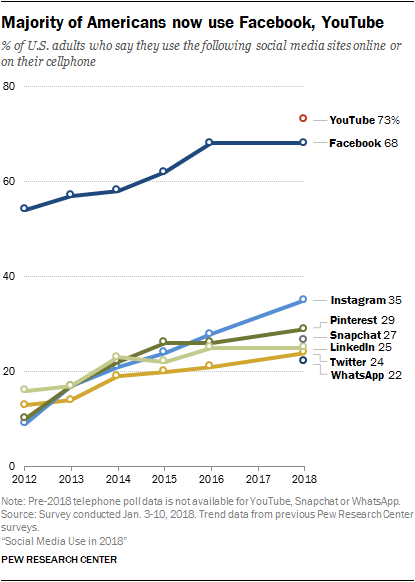
\includegraphics[width=\linewidth]{mass_media.png}
  \caption{The increase of the usage of the different kinds of social networks in the USA}
  \label{discussion.fig.media}
\end{figure}

Many worried about its threat to the individualism, since the other-directed people could easily be influenced by the mass media. Also written by David Riesman in the preface of the book ``The Lonely Crowd'', the gravest concern of the authors about the mass media, however, is not their long-run impact on culture, but the fact that the press, the news, the magazines, and particularly the newsreels have become far more ethnocentric and less parochial, which somewhat cover more foreign news, and only to smother it in the self-serving slogans and misleading the crowd. Edward W. Said also suggested that, ``despite the variety and the differences, and however much we proclaim the contrary, what the media produce is neither spontaneous nor completely ``free'': ``news'' does not just happen, pictures and ideas do not merely spring from reality into our eyes and minds, truth is not directly available, we do not have unrestrained variety at our disposal.'' In this information-saturated world, where the information could be both helpful and misleading, we need all the information we can get about all the information we are receiving and need to learn to pick the information we need and worth trusting, meanwhile, to be aware of the faking possibilities and think critical. 
% For example, as the online shopping is very popular and convenient, the ratings and reviews for a good are more and more important for the customers, which is also known by the sellers. Thereafter, they hire someone to rate the product high and write recommendations and compliments for the product, though it works not the same as is described. One one hand, the rating and reviewing system could help us to decide which to buy, on the other hand, some fake and misleading information may lead to the waste of money and time. 






 


			





\pagebreak

\emergencystretch 1.5em
%\printbibliography[heading=bibintoc]
\bibliographystyle{apacite}
\bibliography{amycao.bib}




%\begin{declaration}
%\thispagestyle{empty}
%\addchaptertocentry{\authorshipname} 

%Ich versichere hiermit an Eides Statt, dass ich die von mir eingereichte Bachelor‐Arbeit bzw. die von mir namentlich gekennzeichneten Teile selbständig verfasst und ausschließlich die angegebenen Hilfsmittel benutzt habe.
% \\
% \\
% \\
% \noindent Signed:\\
% \rule[0.5em]{25em}{0.5pt} % This prints a line for the signature
 
% \noindent Date: Saarbrücken, den 16.04.2018\\
% \rule[0.5em]{25em}{0.5pt} % This prints a line to write the date
% \end{declaration}

\end{document}  
%----------------------------------------------------------------------------------------

